\chapter{Image matching}
\label{chap:image-matching}


\section{Introduzione}
Quando confrontiamo due immagini, una domanda che sorge spontanea \`e la seguente: quando e sotto quali condizioni due immagini possono essere definite uguali o simili?\par
Questo capitolo affronta l'argomento del confronto d'immagini e in particolare quello che consente di localizzare una data sotto-immagine (\textit{template}) all'interno di un'immagine pi\`u grande (\textit{scene}). La difficolt\`a di queste operazioni sta nel tipo di trasformazione geometrica subita dal template all'interno dell'immagine in esame, che pu\`o essere di vari tipi:
\begin{itemize}
	\item \textit{Scala} $\gets$ Ridimensionamento dell'immagine
	\item \textit{Traslazione} $\gets$ Spostamento dell'immagine, in direzione $(x, y)$ di un determinato \textit{shift} $(t_{x}, t_{y})$
	\item \textit{Rotazione} $\gets$ Rotazione dell'immagine di un determinato angolo $\theta$
	\item \textit{Trasformazione affine} $\gets$ Trasformazione geometrica in cui tutte le linee parallele dell'immagine originale rimangono parallele nell'immagine trasformata, ma possono cambiare angoli e lunghezze
	\item \textit{Trasformazione prospettica} $\gets$ Trasformazione geometrica 3D non affine, che conserva solo la rettilinearit\`a, ovvero trasforma linee in linee e figure concave (convesse) in figure concave (convesse)
\end{itemize}
Possiamo affermare che le \textit{trasformazioni affini} sono un sottoinsieme delle \textit{trasformazioni prospettiche} (\textit{omografie}), in quanto quest'ultime consentono di mappare linee parallele in non parallele e viceversa.\par
In figura \ref{fig:image-matching-transformations} un esempio delle trasformazioni descritte:
\pgfplotsset{compat=1.9}
\definecolor{zzttqq}{rgb}{0.6,0.2,0}
\begin{figure}[H]
	\centering
	\vspace*{-125pt}
	\begin{tikzpicture}[line cap=round,line join=round,>=triangle 45,x=0.65cm,y=0.65cm]
		\clip(-13.507354775873502,-4.01960764723451) rectangle (13.54377717739078,14.287457239105523);
		\fill[line width=2pt,color=zzttqq,fill=zzttqq,fill opacity=0.11] (-11.46941052470137,4.683064942964992) -- (-9.451639148270317,4.679101384021924) -- (-9.44767558932725,6.696872760452977) -- (-11.465446965758302,6.7008363193960445) -- cycle;
		\filldraw[line width=2pt,color=zzttqq,fill=zzttqq,fill opacity=0.11] (-8.06160190949523,3.6263801010405947) -- (-6.043830533064177,3.6224165420975263) -- (-6.03986697412111,5.6401879185285795) -- (-8.05763835055216,5.644151477471647) -- cycle;
		\filldraw[line width=2pt,color=zzttqq,fill=zzttqq,fill opacity=0.11] (-3.721265372279725,4.314294102722081) -- (-2.0661304203545825,5.468393460775676) -- (-3.2202297784081777,7.123528412700817) -- (-4.875364730333318,5.9694290546472235) -- cycle;
		\fill[line width=2pt,color=zzttqq,fill=zzttqq,fill opacity=0.11] (0.09746256390296704,6.600075014105602) -- (2.1844151267036294,6.098149714191514) -- (1.154147405827353,4.381036846064381) -- (-0.9063880359251993,4.909379267026575) -- cycle;
		\fill[line width=2pt,color=zzttqq,fill=zzttqq,fill opacity=0.11] (3.5845225422534424,4.090448514535173) -- (5.829977831342763,5.35847032484444) -- (4.614790263129719,7.577508492885656) -- (3.241099968628017,6.943497587731023) -- cycle;
		\draw [line width=2pt,color=zzttqq] (-11.46941052470137,4.683064942964992)-- (-9.451639148270317,4.679101384021924);
		\draw [line width=2pt,color=zzttqq] (-9.451639148270317,4.679101384021924)-- (-9.44767558932725,6.696872760452977);
		\draw [line width=2pt,color=zzttqq] (-9.44767558932725,6.696872760452977)-- (-11.465446965758302,6.7008363193960445);
		\draw [line width=2pt,color=zzttqq] (-11.465446965758302,6.7008363193960445)-- (-11.46941052470137,4.683064942964992);
		\draw [line width=2pt,color=zzttqq] (0.09746256390296704,6.600075014105602)-- (2.1844151267036294,6.098149714191514);
		\draw [line width=2pt,color=zzttqq] (2.1844151267036294,6.098149714191514)-- (1.154147405827353,4.381036846064381);
		\draw [line width=2pt,color=zzttqq] (1.154147405827353,4.381036846064381)-- (-0.9063880359251993,4.909379267026575);
		\draw [line width=2pt,color=zzttqq] (-0.9063880359251993,4.909379267026575)-- (0.09746256390296704,6.600075014105602);
		\draw [line width=2pt,color=zzttqq] (3.5845225422534424,4.090448514535173)-- (5.829977831342763,5.35847032484444);
		\draw [line width=2pt,color=zzttqq] (5.829977831342763,5.35847032484444)-- (4.614790263129719,7.577508492885656);
		\draw [line width=2pt,color=zzttqq] (4.614790263129719,7.577508492885656)-- (3.241099968628017,6.943497587731023);
		\draw [line width=2pt,color=zzttqq] (3.241099968628017,6.943497587731023)-- (3.5845225422534424,4.090448514535173);
		\end{tikzpicture}
		\vspace*{-125pt}
	\caption{Trasformazioni geometriche (originale, traslazione, rotazione, affine e prospettica)}
	\label{fig:image-matching-transformations}
\end{figure}\par
Le sezioni seguenti descrivono vari metodi testati nella libreria QI-OCR per la localizzazione di un documento, a partire da una data immagine \textit{template}.


\section{Template matching}
L'approccio pi\`u semplice al quale si pu\`o pensare, molto simile a quello utilizzato nella \textit{convoluzione}, riguarda lo scorrimento dell'immagine \textit{template} sull'immagine di input, per confrontare il template e l'area dell'immagine originale coperta dal template stesso. L'output di questa operazione \`e ancora un'immagine, in scala di grigi, in cui ogni pixel denota il grado di similitudine dei suoi "vicini" con il template. La scelta dell'area intorno al pixel di intensit\`a massima, nell'immagine prodotta, dar\`a cos\`i il risultato cercato.\par
Il punto cruciale di questa tecnica sta nel metodo di confronto fra pixel scelto, che potrebbe essere, ad esempio, la misura di \textit{distanza euclidea}. Consideriamo $d_{E}(r, s)$ come la distanza euclidea tra l'immagine template $T$ e l'immagine in input $I$, nella posizione $(r, s)$:
\begin{equation}
	\label{eq:euclidean-distance}
	d_{E}(r, s) = \sqrt{\sum_{(i, j)\in T} (I(r + i, s + j) - T(i, j))^{2}}
\end{equation}
A questo punto, per trovare la posizione di \textit{match} migliore, \`e necessario minimizzare il quadrato di $d_{E}(r, s)$:
\begin{equation}
	\label{eq:euclidean-distance-squared}
	\begin{split}
		& d_{E}^{2}(r, s) = \sum_{(i, j)\in T} (I(r + i, s + j) - T(i, j))^{2} = \\
		& = \underbrace{\sum_{(i, j)\in T} I^{2}(r + i, s + j)}_{A(r,s)} + \underbrace{\sum_{(i, j)\in T} T^{2}(i, j)}_{B} - 2 \cdot \underbrace{\sum_{(i, j)\in T} I(r + i, s + j) \cdot T(i, j)}_{C(r,s)}  
	\end{split}
\end{equation}
Possiamo notare che ci siamo appena ricondotti alla risoluzione di un problema di \textit{correlazione lineare}, come descritto in \ref{sec:math-convolution}. In particolare, considerando i due termini $A(r,s)$ e $B$ come costanti\footnote{Sfortunatamente, l'assunzione che il termine $A(r,s)$ sia costante non vale generalmente ed \`e per questo necessario l'utilizzo di nozioni pi\`u avanzate, come il \textit{coefficiente di correlazione}.}, otteniamo proprio l'equazione \ref{eq:correlation}.\par
Il problema principale del \textit{template matching} \`e la poca resistenza a trasformazioni geometriche, anche semplici. Un modo per evitare il presentarsi di questi problemi \`e quello di utilizzare diverse immagini \textit{template}, scalate e ruotate, a discapito dell'efficienza di esecuzione.


\section{Feature matching}
Questo approccio si basa sull'utilizzo di particolari punti di un'immagine, denominati \textit{keypoints} (letteralmente \textit{punti chiave}), che possono godere di elevata robustezza e stabilit\`a per quanto riguarda trasformazioni geometriche e fotometriche (illuminazione e contrasto). I \textit{keypoints} vengono identificati da specifiche \textit{feature} dell'immagine, quali bordi e contorni, e vengono associati a particolari \textit{descrittori locali}, che codificano informazioni di interesse intorno a ciascun \textit{keypoint}. Una volta individuati \textit{keypoints} e \textit{descrittori} del template e dell'immagine in input \`e possibile computare un \textit{matching}, che consiste nell'individuare l'associazione fra le varie \textit{feature} delle due immagini.\par
Esistono vari algoritmi di \textit{feature matching}, come \textit{KNN} (\textit{K-Nearest-Neighbors}), che prevedono l'utilizzo dei due seguenti metodi principali:
\begin{itemize}
	\item \textit{Esaustivo} $\gets$ Ritorna il miglior \textit{match} (\textit{brute force}) o i migliori $K$ \textit{match}, per ciascuna \textit{feature}, in senso assoluto
	\item \textit{Approssimato} $\gets$ \`E basato sull'utilizzo di algoritmi efficienti di ricerca \textit{nearest neighbor} approssimata\footnote{La libreria \textit{OpenCV} si appoggia alla libreria esterna \textit{FLANN (Fast Library for Approximate Nearest Neighbors)} per questo tipo di operazioni.}, che vengono utilizzati solo per insiemi di \textit{feature} di dimensioni elevate 
\end{itemize}\par
Alcuni degli algoritmi pi\`u conosciuti e utilizzati per il calcolo di \textit{keypoints} e \textit{descrittori} sono \textit{SIFT (Scale Invariant Feature Transform)} \cite{bib:sift}, \textit{SURF (Speeded Up Robust Feature)} \cite{bib:surf}, \textit{AKAZE (Accelerated KAZE \cite{bib:kaze})} \cite{bib:akaze}, \textit{BRISK (Binary Robust Invariant Scalable Keypoints)} \cite{bib:brisk}, \textit{ORB (Oriented FAST and Rotated BRIEF)} \cite{bib:orb} e altri.


\section{Shape detection}
Nel caso specifico della libreria QI-OCR, le operazioni descritte di \textit{template matching} e \textit{feature matching} non sono le sole applicabili per la localizzazione del documento d'identit\`a nell'immagine in input. Infatti, considerando le varie tipologie di documenti presenti in territorio internazionale, \`e possibile osservare una caratteristica comune a tutti, ovvero la loro \textit{forma rettangolare}, pi\`u o meno stondata ai vertici. Questo \textit{pattern} consente quindi l'esplorazione di strategie alternative a quelle gi\`a menzionate, permettendo l'utilizzo di alcuni algoritmi di \textit{shape detection}.\par
In particolare, la procedura utilizzata prevede l'individuazione dei bordi presenti nell'immagine e la selezione del contorno di forma approssimativamente rettangolare di area massima, supponendo, appunto, che tale forma sia proprio il documento cercato. La supposizione appena effettuata \`e consistente, poich\`e \`e possibile presumere che anche nel caso in cui il documento d'identit\`a abbia subito svariate trasformazioni geometriche e la qualit\`a della scansione/fotografia non sia eccelsa, questo sia comunque l'oggetto prevalente all'interno dell'immagine.\par
Dunque, nelle seguenti sezioni analizzeremo vari metodi di \textit{edge detection}.

\subsection{Edge detection basata sul gradiente}
Questi metodi di rilevamento dei bordi si basano sul concetto di \textit{derivata} di un'immagine, dato che questo consente l'analisi di cambiamenti in intensit\`a all'interno di una funzione, ovvero la presenza di un bordo all'interno di un'immagine. Solitamente, la derivata parziale $f_{x}=\frac{\partial f}{\partial x}(x, y)$ di una funzione $f(x, y)$ pu\`o essere calcolata solamente se questa \`e  definita nel \textit{continuo}, mentre non \`e definita nel caso \textit{discreto}. Dunque, data una funzione discreta $h(x, y)$, la sua derivata parziale $\frac{\partial h}{\partial x}$ in un punto $(u, v)$ pu\`o essere approssimata interpolando una retta tra i valori vicini $(u + 1, v)$ e $(u - 1, v)$, ottenendo:
\begin{equation}
	\frac{\partial h}{\partial x}(u, v) = \frac{h(u + 1, v) - h(u - 1, v)}{2}
	\label{eq:image-derivative}
\end{equation}
In questo esempio, l'approssimazione della derivata riguarda la direzione orizzontale, lungo l'asse delle ascisse, ma lo stesso metodo pu\`o essere applicato in direzione verticale, per stimare la derivata lungo l'asse delle ordinate.\par
A questo punto, possiamo definire il gradiente di un'immagine $I$ in posizione $(u, v)$ come il vettore contenente le derivate parziali rispetto ai due assi $x$, $y$:
\begin{equation}
	\nabla I(u, v) = 
		\begin{bmatrix}
			I_{x}(u, v) \\ I_{y}(u, v)
		\end{bmatrix}
	\label{eq:image-gradient}
\end{equation}
Dato che il gradiente \`e un vettore, questo avr\`a modulo e direzione\footnote{La direzione del bordo in posizione $(u, v)$ \`e perpendicolare alla direzione del gradiente nella stessa posizione.}:
\begin{equation}
	|\nabla I(u, v)| = \sqrt{I_{x}^{2}(u, v)+I_{y}^{2}(u, v)}
	\label{eq:image-gradient-magnitude}
\end{equation}
\begin{equation}
	\theta (u, v) = \arctan{\frac{I_{x}(u, v)}{I_{y}(u, v)}}
	\label{eq:image-gradient-direction}
\end{equation}\par
Per computare il gradiente di un'immagine, nella pratica viene effettuata una convoluzione con dei particolari filtri. Per esempio, utilizzando il filtro di \textit{Sobel-Feldman}:\\
\vspace*{15pt}
\noindent\begin{minipage}{.5\linewidth}
	\begin{equation}
		I_{x} = I * 
			\begin{pmatrix}
				-1 & 0 & 1 \\
				-2 & 0 & 2\\
				-1 & 0 & 1
			\end{pmatrix},
		\label{eq:sobel-x}
	\end{equation}
\end{minipage}%
\begin{minipage}{.5\linewidth}
	\begin{equation}
		I_{y} = I * 
			\begin{pmatrix}
				-1 & -2 & -1 \\
				0 & 0 & 0\\
				1 & 2 & 1
			\end{pmatrix},
		\label{eq:sobel-y}
	\end{equation}
\end{minipage}\\
oppure quello di \textit{Prewitt} \cite{bib:prewitt}:\\
\noindent\begin{minipage}{.5\linewidth}
	\begin{equation}
		I_{x} = I * 
			\begin{pmatrix}
				-1 & 0 & 1 \\
				-1 & 0 & 1\\
				-1 & 0 & 1
			\end{pmatrix},
		\label{eq:prewitt-x}
	\end{equation}
\end{minipage}%
\begin{minipage}{.5\linewidth}
	\begin{equation}
		I_{y} = I * 
			\begin{pmatrix}
				-1 & -1 & -1 \\
				0 & 0 & 0\\
				1 & 1 & 1
			\end{pmatrix},
		\label{eq:prewitt-y}
	\end{equation}
\end{minipage}


\subsection{Canny edge detector}
L'operatore proposto da Canny \cite{bib:canny} per il rilevamento dei bordi \`e tutt'ora uno dei pi\`u utilizzati e viene considerato lo \textit{stato dell'arte} in questo campo. L'algoritmo \`e suddiviso in 3 passi:
\begin{enumerate}
	\item \textit{Pre-processing} $\gets$ Rimozione del \textit{noise} con un \textit{filtro di Gauss} di dimensione $\sigma$ e calcolo del gradiente tramite il \textit{filtro di Sobel}
	\item \textit{Localizzazione dei bordi} $\gets$ Assottigliamento dei bordi con una procedura di \textit{nms} (\textit{non-maxima-suppression}). Vengono mantenuti solamente i punti di massimo locale, nella direzione del gradiente
	\item \textit{Sogliatura con isterisi e tratteggio dei bordi} $\gets$ La \textit{sogliatura con isterisi} prevede l'utilizzo di due valori di soglia, \vars{thresh-low} e \vars{thresh-high}. Per ciascun punto $(u, v)$, se $|\nabla I(u, v)| \leq \vars{thresh-low}$ allora il punto viene automaticamente scartato, mentre se $|\nabla I(u, v)| \geq \vars{thresh-high}$ allora il punto viene automaticamente accettato come parte di un contorno. Nel caso in cui $\vars{thresh-low} < |\nabla I(u, v)| < \vars{thresh-high}$, allora il punto viene accettato solo se \textit{connesso} a un punto $(u', v')$ tale che $|\nabla I(u', v')| \geq \vars{thresh-high}$
\end{enumerate}\par
L'operatore \textit{Canny} permette di ottenere dei buoni risultati, con un impiego di risorse relativamente basso, ma ha lo svantaggio di dipendere dai 3 parametri $\sigma$, \vars{thresh-low} e \vars{thresh-high}, strettamente dipendenti dal contesto di applicazione.
\begin{figure}[h]
	\centering
	\resizebox{\textwidth}{!}{
		\subfloat[Input] {%
			\scalebox{0.5}[0.5] {
				\frame{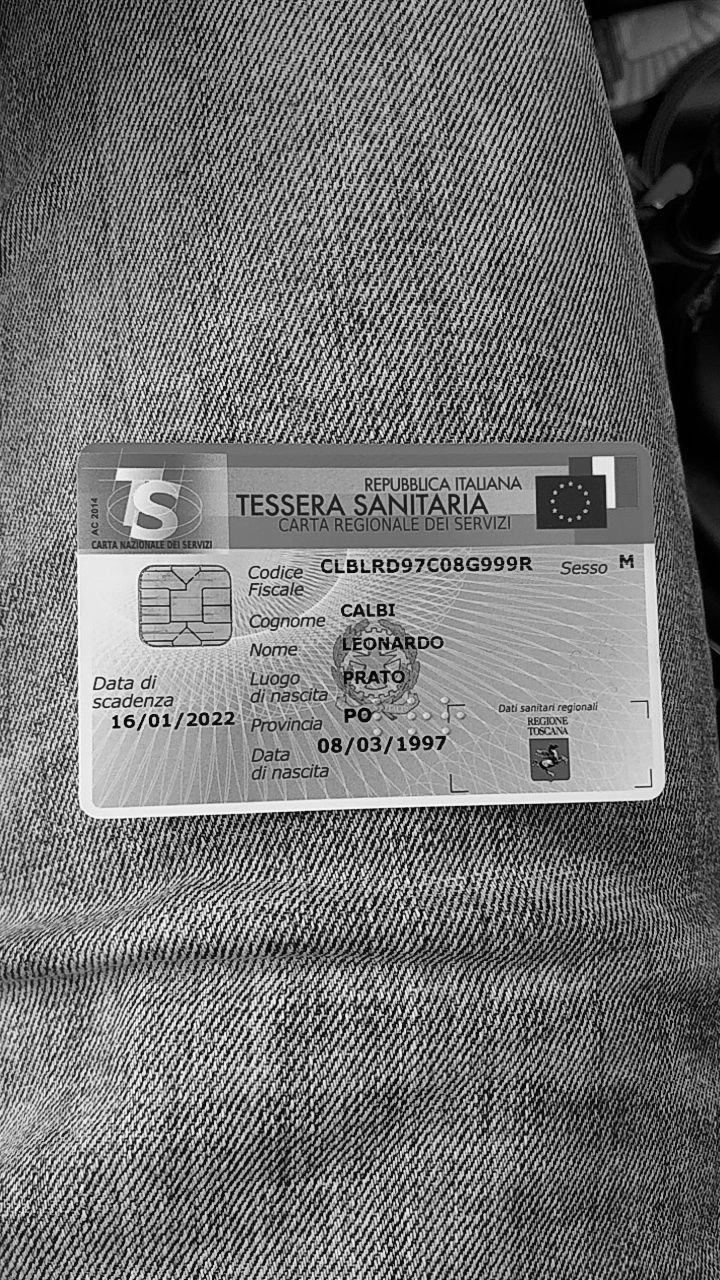
\includegraphics[width=.5\linewidth]{img/canny-hed-input.png}}
			}
		}
		\subfloat[][$\vars{thresh-low}=22$,\newline$\vars{thresh-high}=66$,\newline$\sigma=7$] {%
			\scalebox{0.5}[0.5] {
				\frame{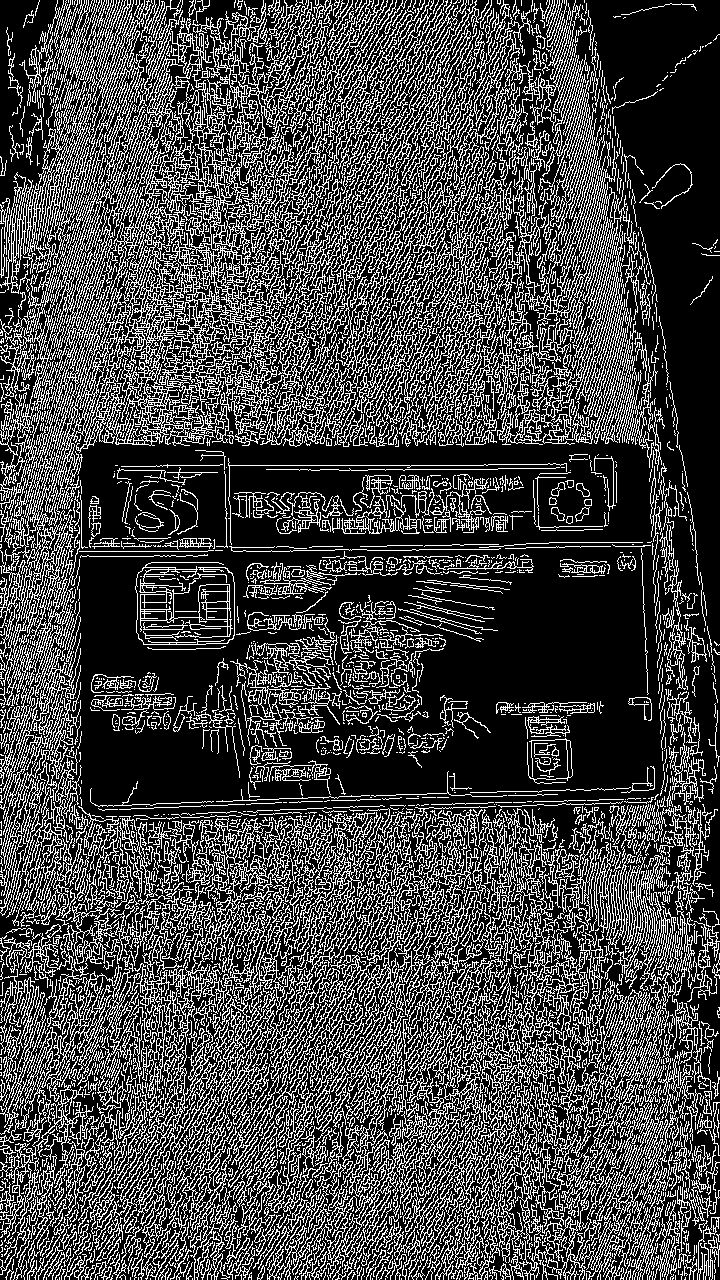
\includegraphics[width=.5\linewidth]{img/canny-min22-sigma7.png}}
			}
		}
		\subfloat[][$\vars{thresh-low}=55$,\newline$\vars{thresh-high}=165$,\newline$\sigma=6$] {%
			\scalebox{0.5}[0.5] {
				\frame{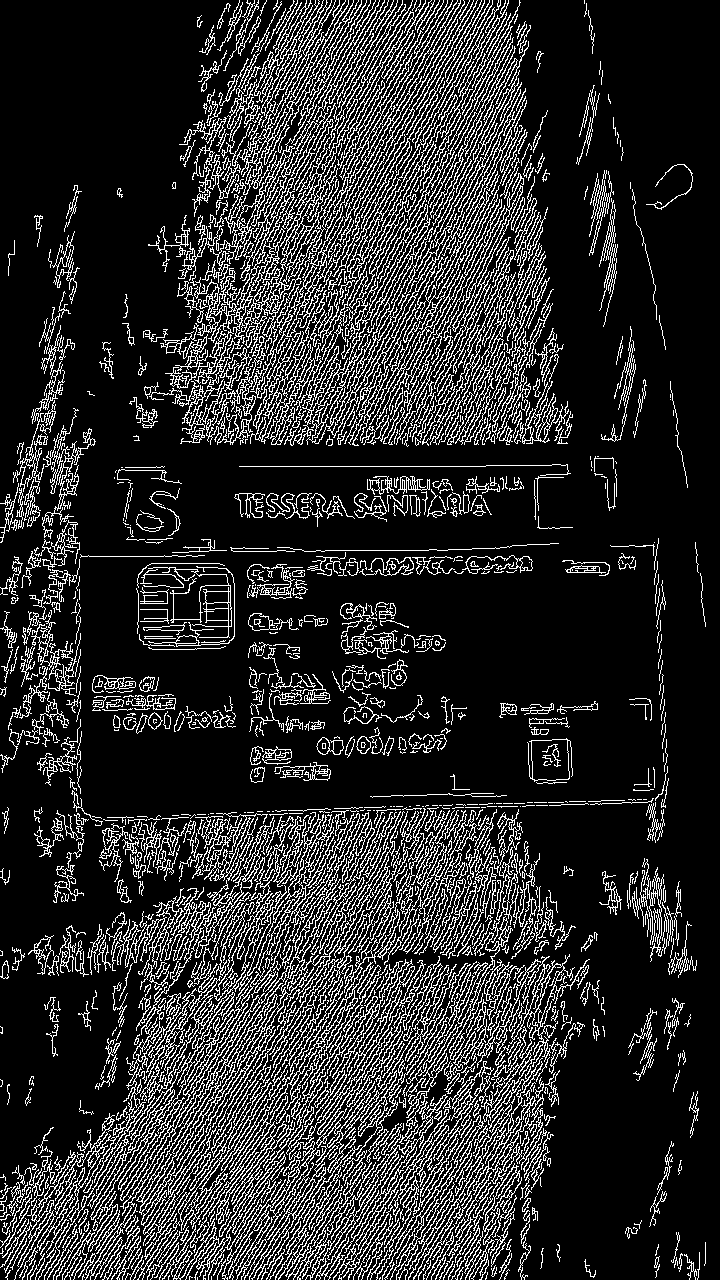
\includegraphics[width=.5\linewidth]{img/canny-min55-sigma6.png}}
			}
		}
		\subfloat[][$\vars{thresh-low}=100$,\newline$\vars{thresh-high}=255$,\newline$\sigma=2$] {%
			\scalebox{0.5}[0.5] {
				\frame{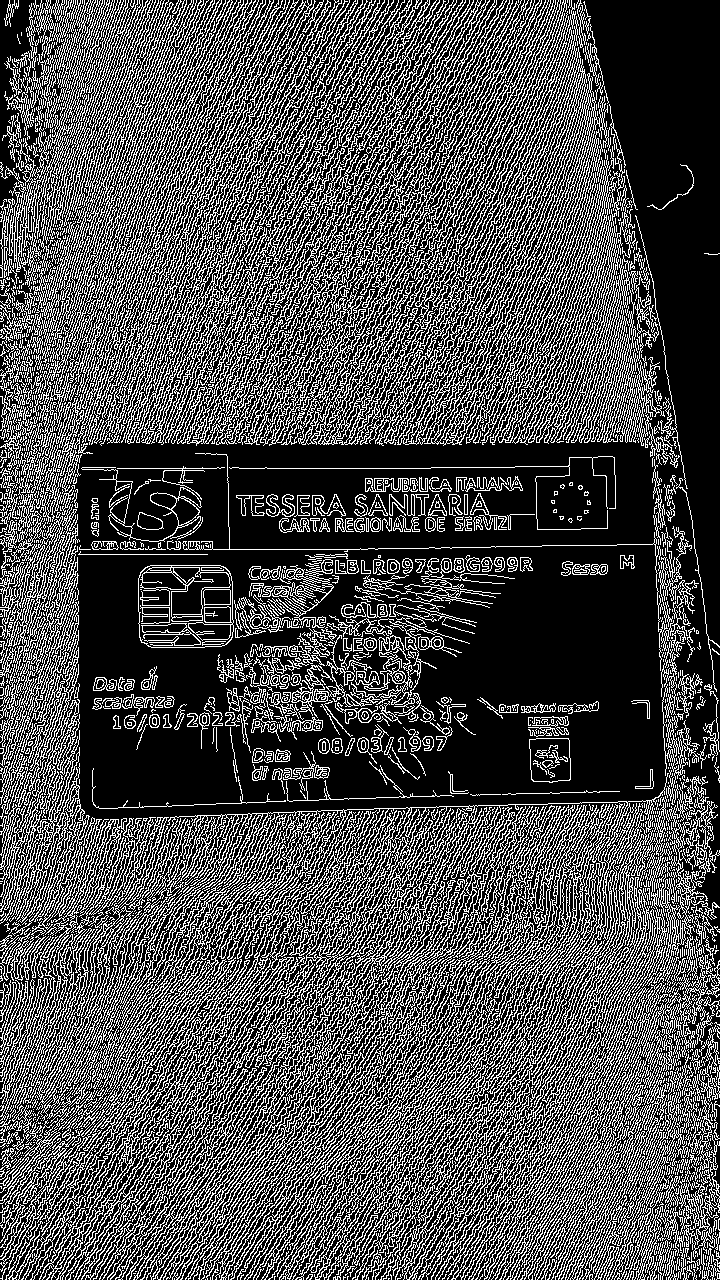
\includegraphics[width=.5\linewidth]{img/canny-min100-sigma2.png}}
			}
		}
	}
	\caption{Operatore \textit{Canny} con diversi parametri} \label{fig:canny}
\end{figure}

\subsection{HED}
L'approccio ideale per i problemi di \textit{edge detection} sarebbe quello di utilizzare un algoritmo che prende in input un'immagine e restituisce un'immagine binaria contenente informazioni sui bordi rilevanti dell'immagine in input, senza dover necessariamente impostare parametri diversi per contesti diversi.
\textit{HED} (\textit{Holistically-nested Edge Detection}) \cite{bib:hed} cerca di superare i limiti dell'operatore \textit{Canny}, tramite l'implementazione di una rete neurale convoluzionale. Le specifiche di questa soluzione non rientrano negli obiettivi di questa tesi, ma nelle figure \ref{fig:canny} e \ref{fig:hed} presentiamo un esempio di immagine processata sia dall'operatore \textit{Canny} che dalla rete \textit{HED}, per poter confrontare i risultati ottenuti.
\begin{figure}[h]
	\centering
	\resizebox{\textwidth}{!}{
		\centering
		\subfloat[Input] {%
			\scalebox{0.5}[0.5] {
				\frame{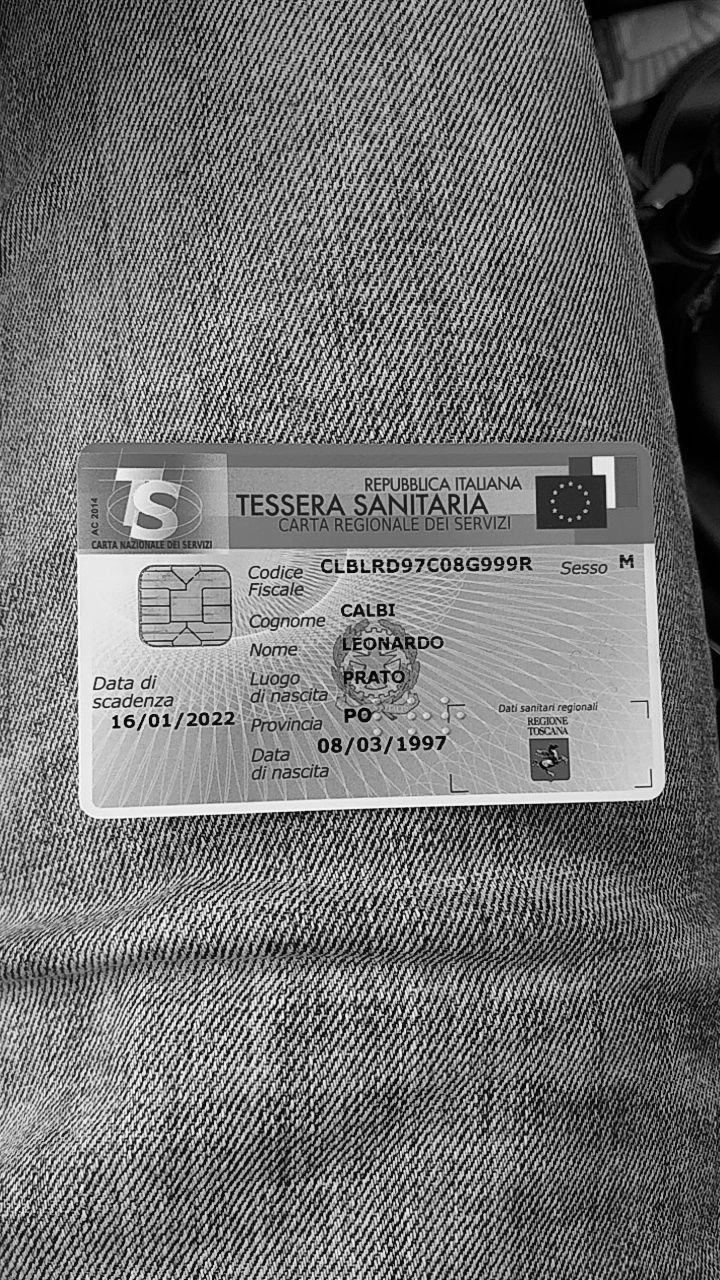
\includegraphics[width=.5\linewidth]{img/canny-hed-input.png}}
			}
		}
		\subfloat[Output] {%
			\scalebox{0.5}[0.5] {
				\frame{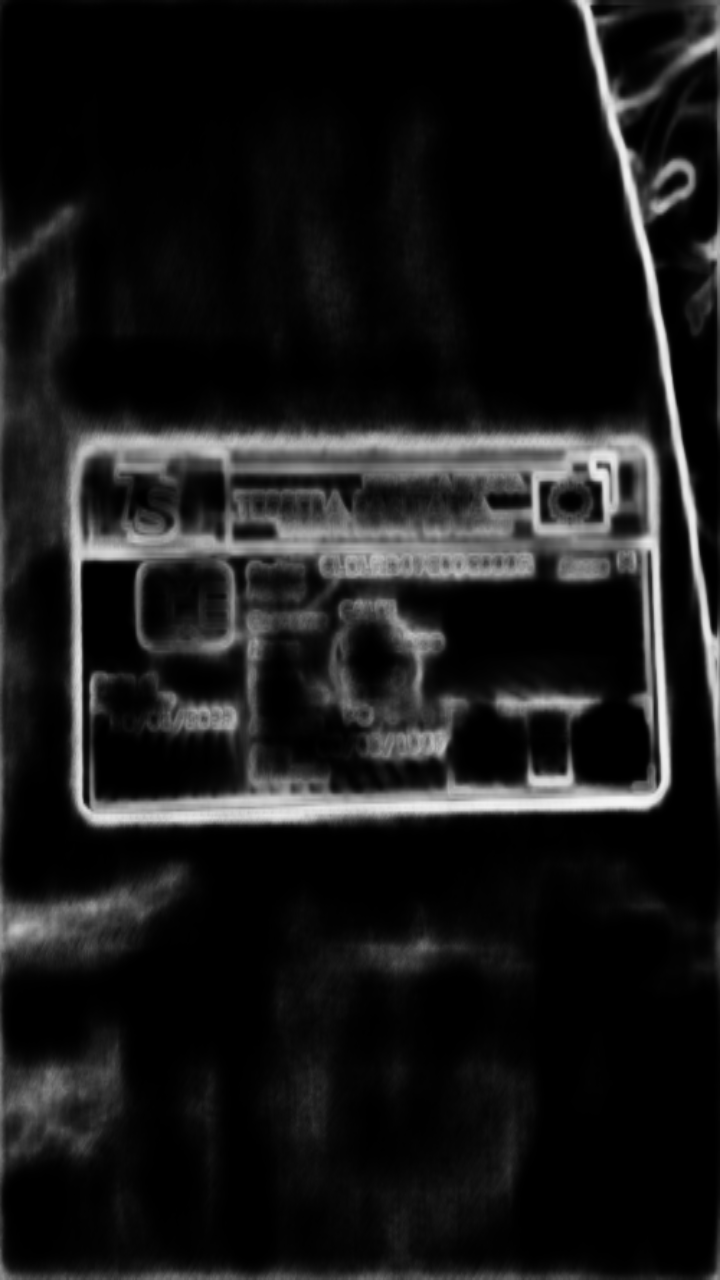
\includegraphics[width=.5\linewidth]{img/hed-output.png}}
			}
		}
		\subfloat[][Output con \textit{dilatazione}] {%
			\scalebox{0.5}[0.5] {
				\frame{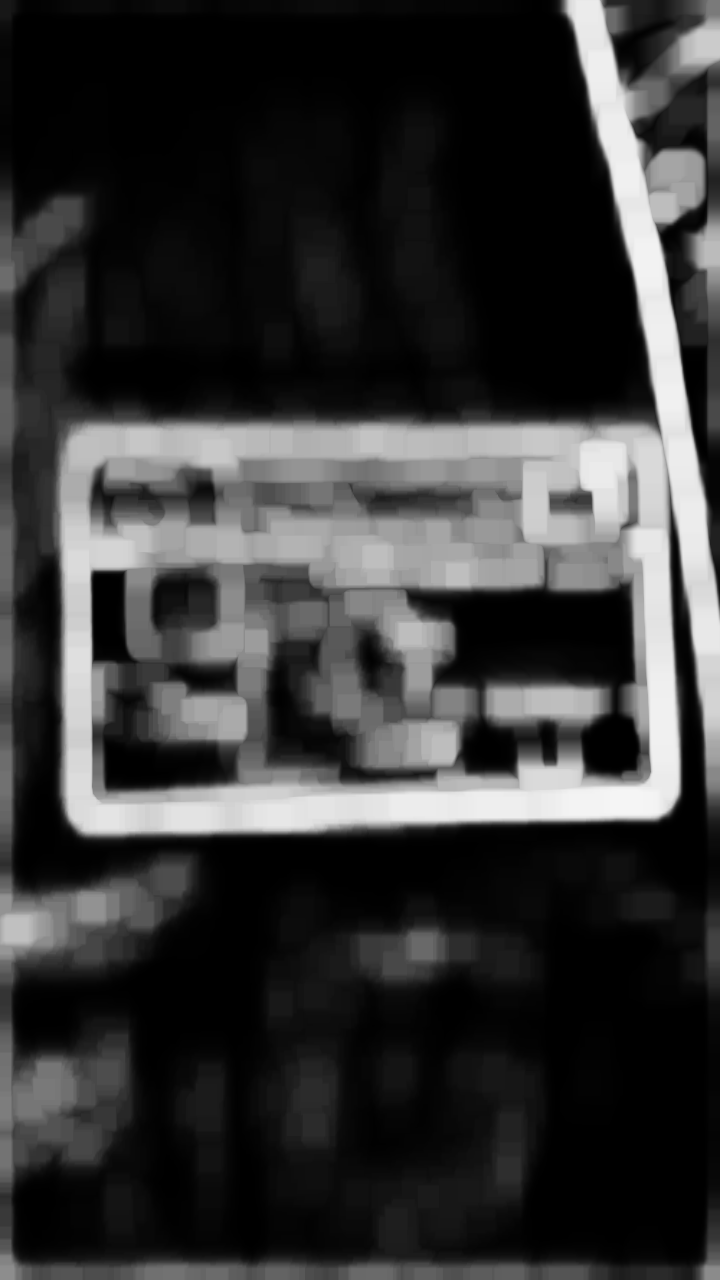
\includegraphics[width=.5\linewidth]{img/hed-output-dilated.png}}
			}
		}
	}
	\caption{Esempio di output della rete \textit{HED}} \label{fig:hed}
\end{figure}

\section{Analisi comparativa}
Inizialmente, la libreria QI-OCR prevedeva il solo utilizzo dell'algoritmo \textit{SIFT} per la localizzazione del documento. A seguito di uno studio comparativo fra gli algoritmi di \textit{image matching} sopra descritti, \`e stato deciso di scartare algoritmi di \textit{template matching}, per favorire quelli di \textit{feature matching} e \textit{shape detection}. In particolare, i primi vengono utilizzati perch\`e invarianti per trasformazioni fotometriche e per tutte le trasformazioni geometriche menzionate, ad eccezione di quelle prospettiche; mentre i secondi vengono utilizzati perch\`e computazionalmente efficienti e possibilmente invarianti anche per trasformazioni prospettiche, anche se non molto resistenti a cambi di illuminazione e/o contrasto dell'immagine.\par
Adesso, l'esecuzione della libreria prevede dunque l'utilizzo congiunto degli algoritmi \textit{SIFT}, \textit{SURF}, \textit{AKAZE} e \textit{BRISK} e della rete \textit{HED}, tramite l'impiego di diversi \textit{thread}. Non appena uno dei thread eseguiti torna il risultato prodotto al \textit{processo padre}, l'esecuzione degli altri thread viene interrotta.\par
L'algoritmo che ha restituito i migliori risultati \`e \textit{AKAZE}, che mantiene all'incirca l'accuratezza di \textit{SIFT}, dimezzando i tempi di esecuzione. L'algoritmo che invece ha restituito i peggiori risultati \`e \textit{ORB}, implementato in fase preliminare e scartato successivamente. Per quanto riguarda \textit{HED} invece, una realizzazione stabile \`e ancora in fase di lavorazione.\par
Infine, per consentire la produzione di \textit{test massivi} e valutare l'accuratezza e la velocit\`a ottenibile con ciascuno degli algoritmi implementati, la libreria risulta configurabile in base al tipo di localizzazione che si intende effettuare. I risultati riportati sono frutto dell'elaborazione da parte della libreria di un insieme di circa 400 documenti d'identit\`a: 

INSERIRE TABELLA RISULTATI (TEMPO +  ACCURATEZZA)
